\section{Evaluation}

\subsection{Implementation and Setup}
We have implement a prototype of our approach named $\alpha$Diff, consisting of two
 components: inputs extractor and neural network model. 
The inputs extractor is a IDAPython \cite{idapython} plug-in to the disassembly tool
 IDA Pro \cite{idapro} and is used to extract the machine code, in/out-degree in call
  graph and calls to imported functions of a function. 
We implement the neural network model with TensorFlow-1.3 \cite{abadi2016tensorflow}
 and Keras-2.0 \cite{chollet2015keras}. 
Our experiments are conducted on a server equipped with two Intel Xeon E5-2650v4
 CPUs (24 cores in total) running at 2.20 GHz, 128 GB memory, 12TB hard drives,
  and 4 NVIDIA Tesla P100 PCIE-16G GPU cards. 
During both training and evaluation, only 1 GPU card was used.

\textbf{Datasets.} In our evaluation, we collect four datasets: 
(1) Dataset \uppercase\expandafter{\romannumeral1} for training the neural network, evaluating the accuracy of the pre-trained model
 and evaluating the effectiveness of hyperparameters in our model; 
(2) Dataset \uppercase\expandafter{\romannumeral2} for evaluating the performance of the model in real-world cross-version settings; 
(3) Dataset \uppercase\expandafter{\romannumeral3} for evaluating the performance in cross-compiler settings; 
(4) Dataset \uppercase\expandafter{\romannumeral4} for evaluating the performance in cross-architecture settings.
\begin{enumerate}
\item \textbf{Dataset \uppercase\expandafter{\romannumeral1}.} 
  The dataset is used to train neural network model and evaluate the accuracy of the pre-trained model. 
  The dataset is consisted of 66,823 pairs of binaries and each of them are two versions of the same
   executable. 
  These binaries comes from two sources:
   (1) GitHub, we collect the releases of some open source projects on GitHub, such as Vim and Git;
    then, we compile them into executables and group two binaries with adjacent version numbers into a pair;
     finally, we obtain 23,524 pairs of binaries; 
  (2) Ubuntu repositories, we collect binaries and their corresponding debug symbol files that coexist on
   Ubuntu 12.04, 14.04 and 16.04; then, we group them into pairs in the similar way. 
   All of these binaries have debug symbols, so that they can provide the ground truth for us. 
   Besides, they are all in x86. We extract samples from the binaries with Inputs Extractor and each sample 
   contains a function’s machine code, in/out-degree in CG and calls to imported functions. 
   For each pair of binaries, we extract machine code samples corresponding to all of changed functions and a small part
    of unchanged ones between two versions. In total, we obtain 2,489,793 samples (pairs of functions) and
     70.6\% of them are function pairs with source code differences. 
     We split Dataset \uppercase\expandafter{\romannumeral1} into three disjoint sets of binary pairs for training (44,526 pairs of binaries, 1,665,025 pairs of functions),
      validation (11,150 pairs of binaries, 417,158 pairs of functions) and testing (11,147 pairs of binaries, 407,610 pairs of functions)
       respectively. During the split, 
    we guarantee that no two binaries from the same project are separated into two different sets among
     training, validation and testing. 
    By doing so, we can examine whether the pre-trained model can generalize to unseen binary files.  
\item \textbf{Dataset \uppercase\expandafter{\romannumeral2}.}
In order to evaluate the performance of $\alpha$Diff in real-world cross-version settings, we construct two sub-datasets:
 (1) We re-extract all function samples including machine code, in/out-degree in CG and calls to imported functions for each binary pair in the testing set of Dataset \uppercase\expandafter{\romannumeral1},
 because we oly extract a portion of functions when constructing Dataset \uppercase\expandafter{\romannumeral1} which is different from the real-world scenarios. 
 In total, the sub-dataset contains 9308 pairs of binaries and more than 1.4 Million user-defined functions.
 (2) In order to compare with BinDiff in classic cross-version setting, we tried to search for standard benchmarks used by other researchers, however,
  we didn't find anyone. So we build a open benchmark which consists of binaries hard to diff and none of the binaries exists in Dataset \uppercase\expandafter{\romannumeral1}.
  Finally, the sub-dataset contains 400 pairs of binaries and 365,374 functions including 176,524 user-defined functions.

\item \textbf{Dataset \uppercase\expandafter{\romannumeral3}.}

\item \textbf{Dataset \uppercase\expandafter{\romannumeral4}.}

\end{enumerate}

\textbf{Training details.} The neural network model is trained using Dataset \uppercase\expandafter{\romannumeral1} as follow. 
We use RMSProp optimizer ...

\subsection{Accuracy}
In this section, we evaluate the accuracy of the pre-trained neural network model (Siamese network embedded with CNN) and $\alpha$Diff in Dataset \uppercase\expandafter{\romannumeral2}.
Before evaluating, we briefly introduce our evaluation metric used in the experiments. 
For two given binaires $BIN_{pre}$ and $BIN_{post}$, not every function in $BIN_{pre}$ has a match in $BIN_{post}$; 
so we use the \textbf{Recall@K} metric \cite{jegou2011product}\cite{song2016deep}. 
Each function (query) in $BIN_{pre}$ first retrieves K nearest neighbors in $BIN_{post}$ and receives 1 if the matched function (with the same function name) is retrieved among the K nearest
 neighbors and 0 otherwise. 
Slightly different to \cite{jegou2011product}\cite{song2016deep}, we furtherly divide the Recall@K number by the total number of matches with same function name between $BIN_{pre}$ and $BIN_{post}$
 and use the result as \textbf{Recall@K} metric.
We evaluate the accuracy of pre-train Siamese network and $\alpha$Diff respectively in Dataset \uppercase\expandafter{\romannumeral2}-1.
 For each binary pair, we compute Recall@1 and Recall@5 respectively. Finally, we compute the mean values among all binary pairs, shown as Table \uppercase\expandafter{\romannumeral1}.
 The Siamese network diffs binaries only with the intra-function feature identified by itself and $\alpha$Diff
  makes comprehensive use of the intra-function feature, inter-function feature and inter-module feature.
  Although both of them performs well in Dataset \uppercase\expandafter{\romannumeral2}-1, 
  Recall@1 mean of $\alpha$Diff is still higher than Siamese network's by 3 permillage. 
  So the global context features are useful and becomes more importanter in the following evaluation.  

Besides, we compare $\alpha$Diff with BinDiff, the state-of-the-art tool specialized in cross-version diffing problem, on Dataset \uppercase\expandafter{\romannumeral2}-2, shown as Table \uppercase\expandafter{\romannumeral2} and Figure \ref{fig_alphadiff_bindiff}.
 As we can see, the binaries in Dataset \uppercase\expandafter{\romannumeral2}-2 are harder to diff than ones in Dataset \uppercase\expandafter{\romannumeral2}-1.
 This is partly beacuse each binary has more functions on average and each function becomes more difficult to distinguish to the others of the same binary.
 In brief, both Siamese network and $\alpha$Diff outperforms BinDiff; the Recall@1 mean of Siamese network is very close to BinDiff's;
 $\alpha$Diff outperforms about 12\% than BinDiff on Recall@1 metric, which means the global context features bring more benefits and are necessary. 
 Because BinDiff only outputs the best match (rank-1) for each function, we can not compute Recall@5 for it. 
 An interesting observation is the gap becomes smaller as K increases, which can be explained as that {\color{red}XXXXXX...}.

   

top-1 accuracy in testing set and the selected smaller benchmark VS BinDiff

\subsection{Hyperparameters}
\subsubsection{the number of negative samples corresponding to a positive sample}

1:1 vs 1:3 vs 1:7 vs 1:15

\subsubsection{embedding size}

64 vs 128 vs 256 vs 512 vs 1024

\subsubsection{distance metric}

euclidean distance vs cosine distance

\subsubsection{pooling algorithm}
max pooling vs average pooling

\subsection{Cross-compiler}


\subsection{Cross-architecture}


\par To Esh \& BinDiff in cross-compiler

\par To BinGo in cross-compiler \& cross-architecture

\par To Genius \& Gemini in cross-architecture vulnerability search


% An example of a floating figure using the graphicx package.
% Note that \label must occur AFTER (or within) \caption.
% For figures, \caption should occur after the \includegraphics.
% Note that IEEEtran v1.7 and later has special internal code that
% is designed to preserve the operation of \label within \caption
% even when the captionsoff option is in effect. However, because
% of issues like this, it may be the safest practice to put all your
% \label just after \caption rather than within \caption{}.
%
% Reminder: the "draftcls" or "draftclsnofoot", not "draft", class
% option should be used if it is desired that the figures are to be
% displayed while in draft mode.
%
%\begin{figure}[!t]
%\centering
%\includegraphics[width=2.5in]{myfigure}
% where an .eps filename suffix will be assumed under latex, 
% and a .pdf suffix will be assumed for pdflatex; or what has been declared
% via \DeclareGraphicsExtensions.
%\caption{Simulation Results.}
%\label{fig_sim}
%\end{figure}

\begin{figure}[!t]
\centering
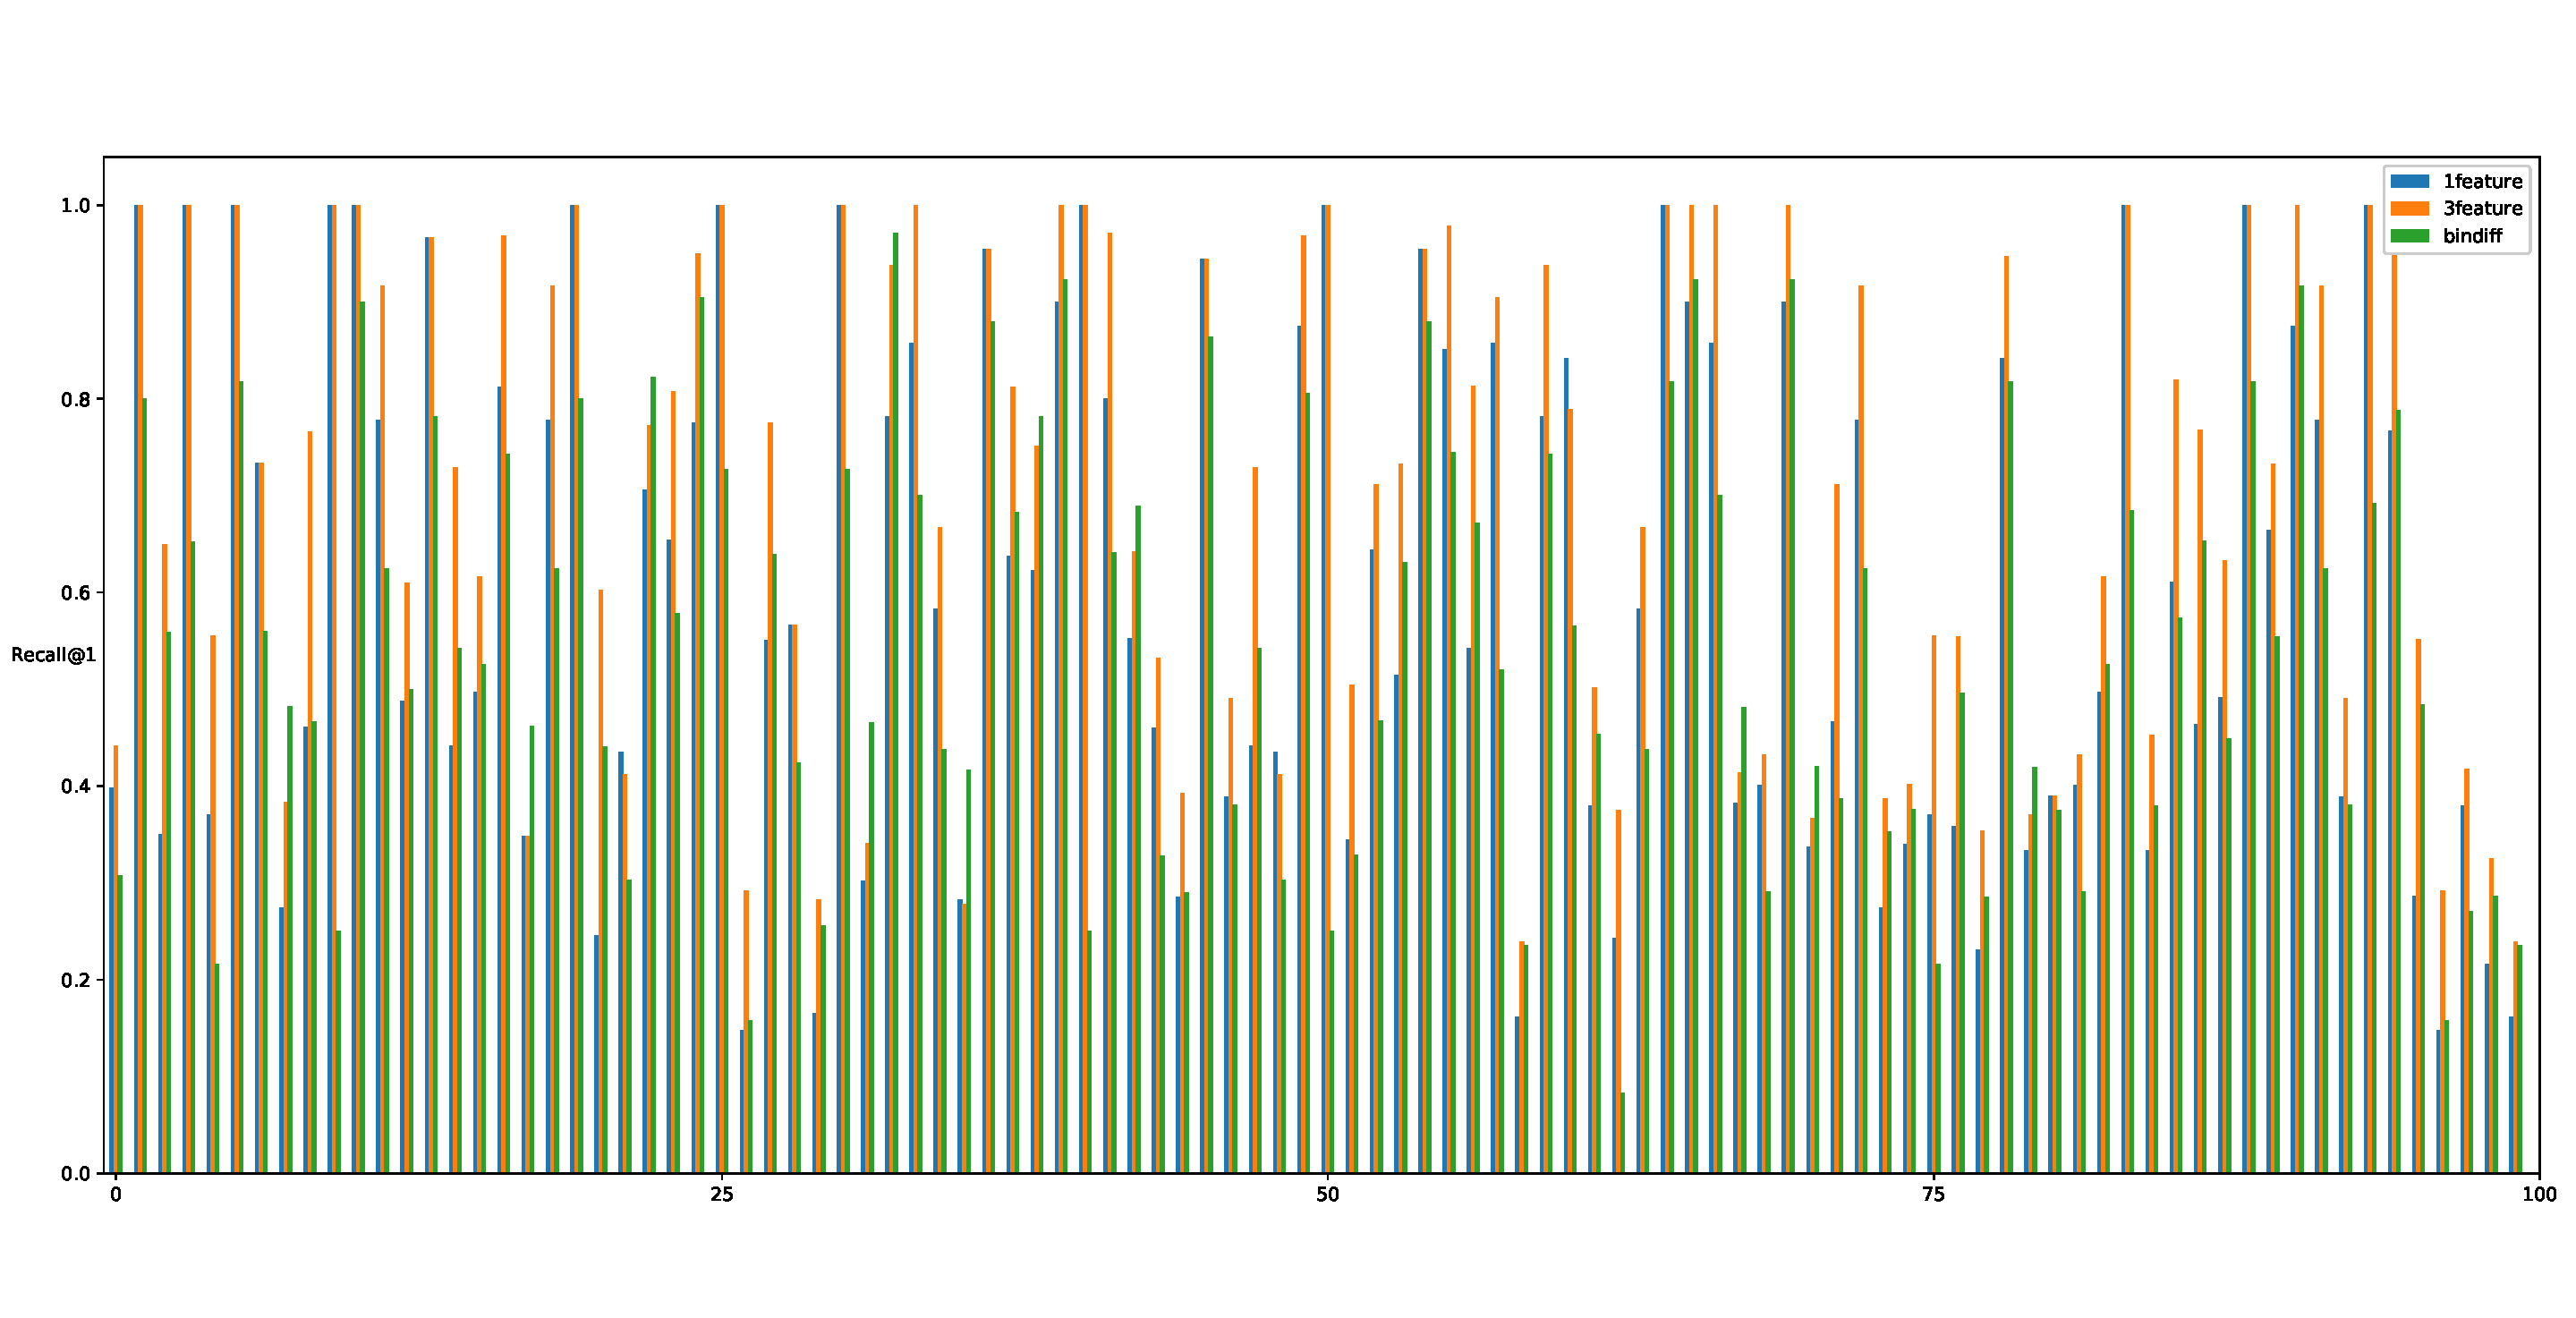
\includegraphics[width=3.5in]{figures/Figure_1.pdf}
% where an .eps filename suffix will be assumed under latex, 
% and a .pdf suffix will be assumed for pdflatex; or what has been declared
% via \DeclareGraphicsExtensions.
\caption{Simulation Results.}
\label{fig_alphadiff_bindiff}
\end{figure}

\begin{figure}[!t]
  \centering
  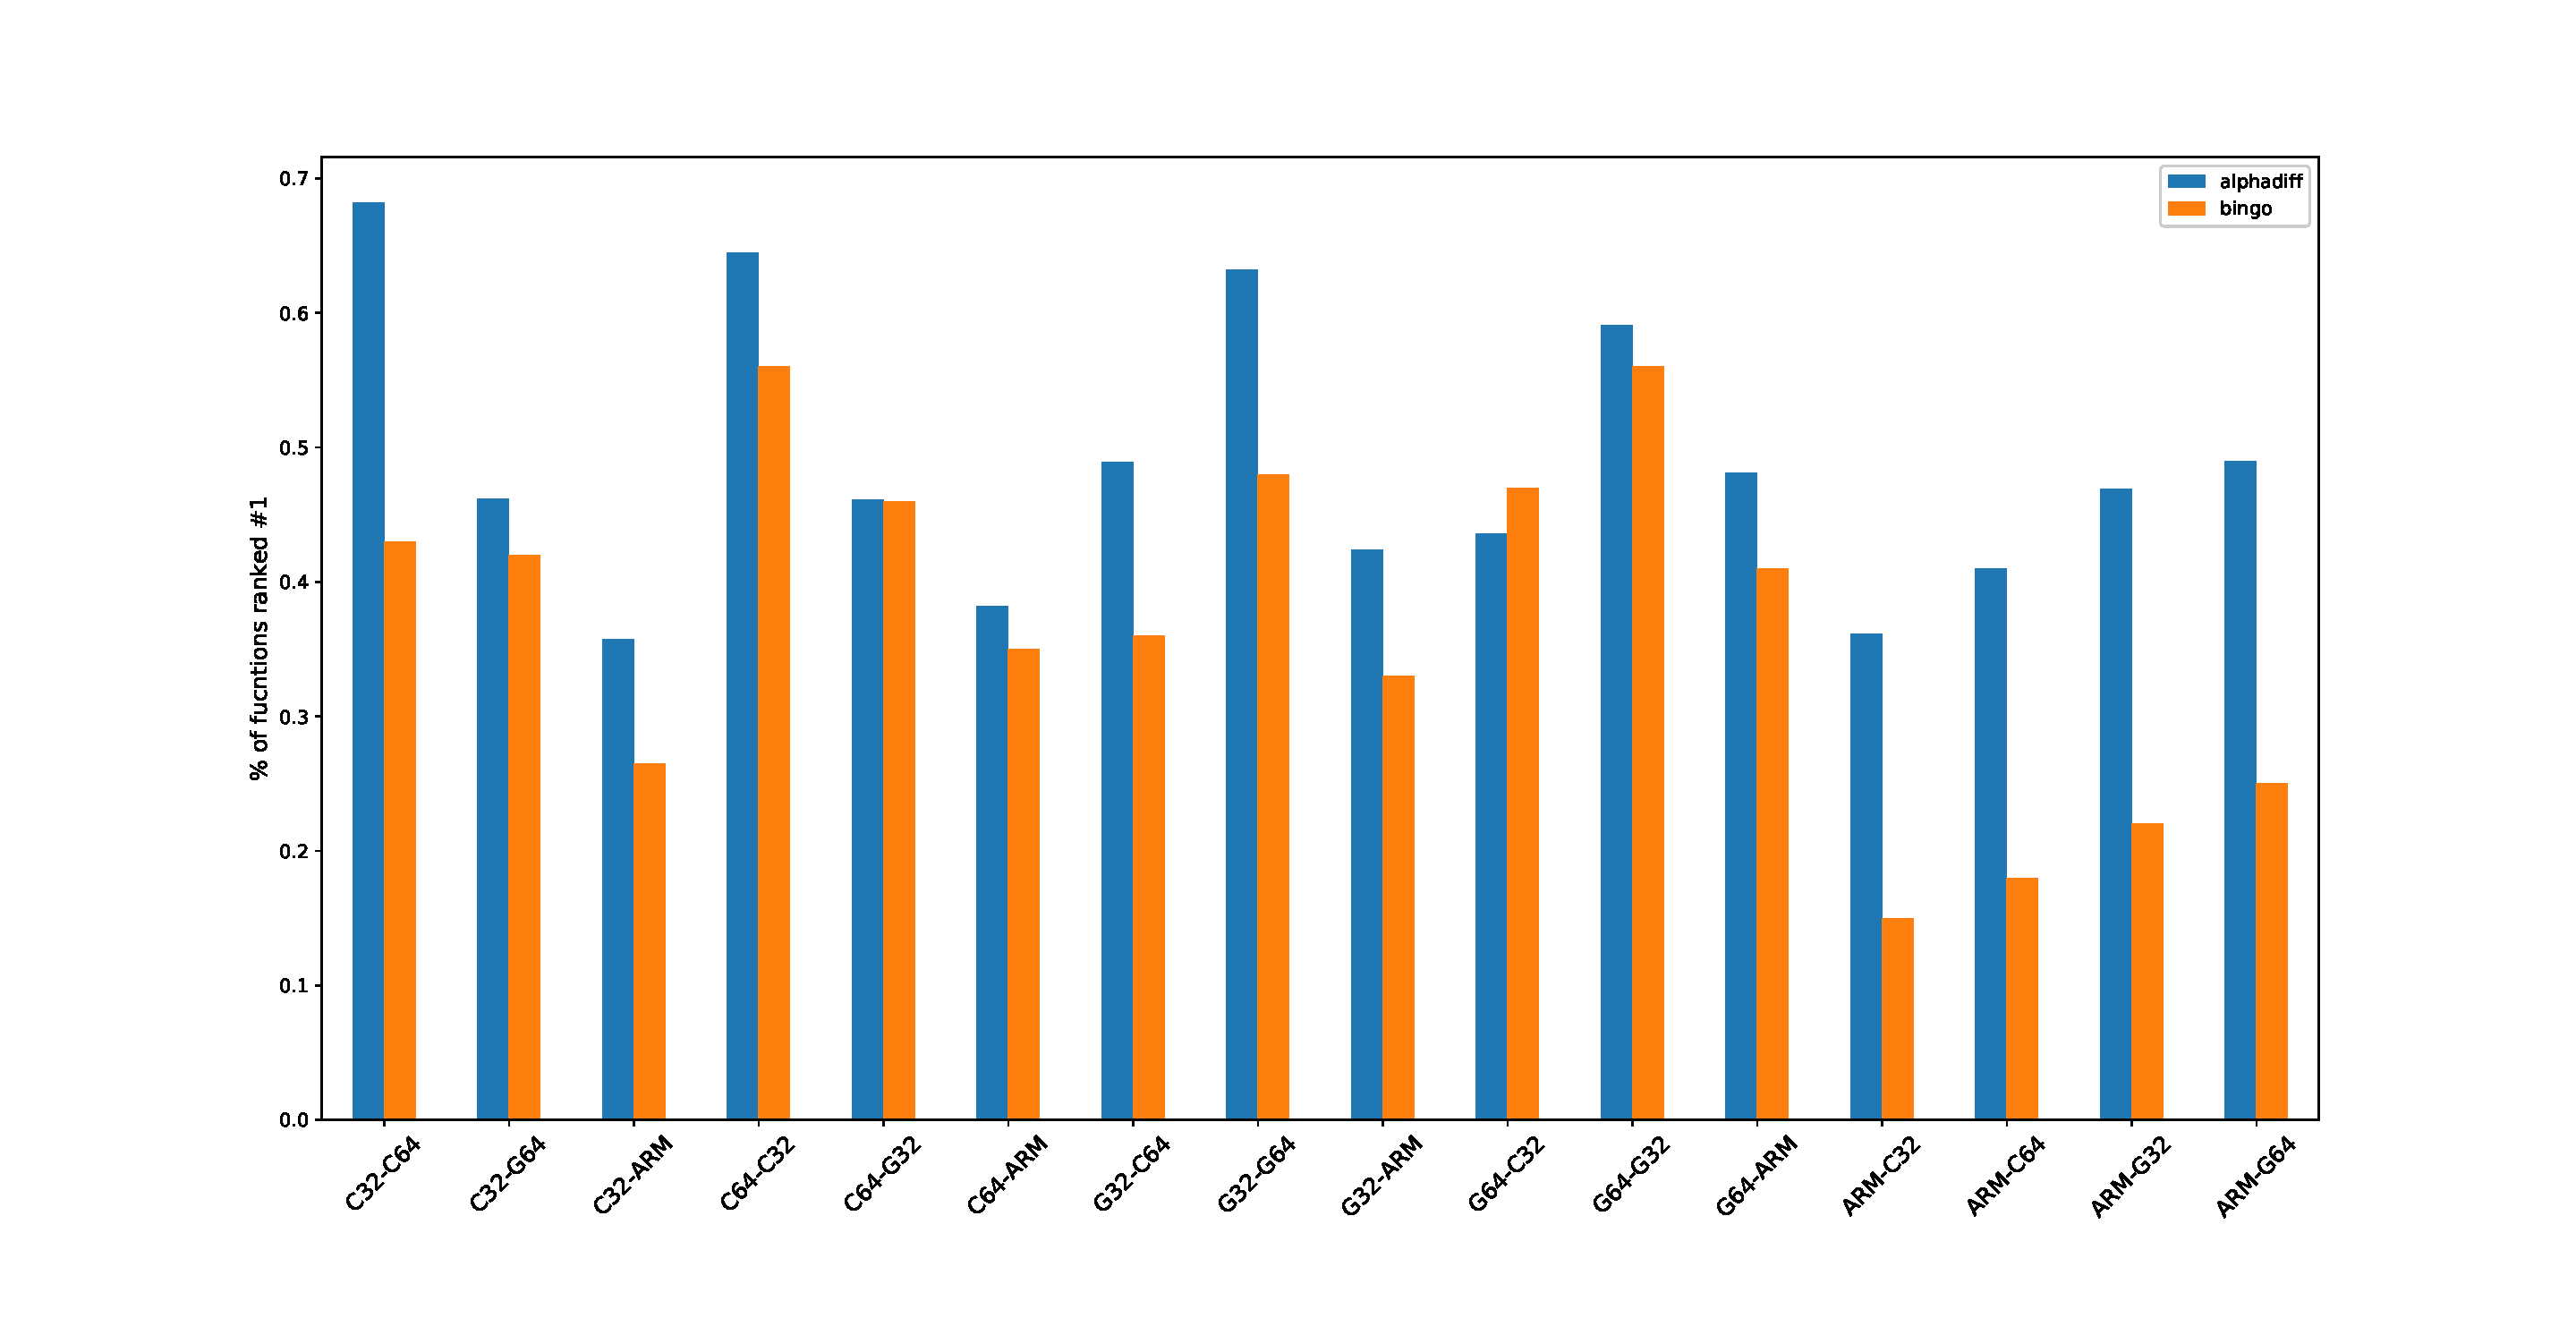
\includegraphics[width=4in]{figures/Figure_2.pdf}
  % where an .eps filename suffix will be assumed under latex, 
  % and a .pdf suffix will be assumed for pdflatex; or what has been declared
  % via \DeclareGraphicsExtensions.
  \caption{Simulation Results.}
  \label{fig_alphadiff_bingo_xcompiler}
  \end{figure}

% Note that IEEE typically puts floats only at the top, even when this
% results in a large percentage of a column being occupied by floats.


% An example of a double column floating figure using two subfigures.
% (The subfig.sty package must be loaded for this to work.)
% The subfigure \label commands are set within each subfloat command,
% and the \label for the overall figure must come after \caption.
% \hfil is used as a separator to get equal spacing.
% Watch out that the combined width of all the subfigures on a 
% line do not exceed the text width or a line break will occur.
%
%\begin{figure*}[!t]
%\centering
%\subfloat[Case I]{\includegraphics[width=2.5in]{box}%
%\label{fig_first_case}}
%\hfil
%\subfloat[Case II]{\includegraphics[width=2.5in]{box}%
%\label{fig_second_case}}
%\caption{Simulation results.}
%\label{fig_sim}
%\end{figure*}
%
% Note that often IEEE papers with subfigures do not employ subfigure
% captions (using the optional argument to \subfloat[]), but instead will
% reference/describe all of them (a), (b), etc., within the main caption.


% An example of a floating table. Note that, for IEEE style tables, the 
% \caption command should come BEFORE the table. Table text will default to
% \footnotesize as IEEE normally uses this smaller font for tables.
% The \label must come after \caption as always.
%
%\begin{table}[!t]
%% increase table row spacing, adjust to taste
%\renewcommand{\arraystretch}{1.3}
% if using array.sty, it might be a good idea to tweak the value of
% \extrarowheight as needed to properly center the text within the cells
%\caption{An Example of a Table}
%\label{table_example}
%\centering
%% Some packages, such as MDW tools, offer better commands for making tables
%% than the plain LaTeX2e tabular which is used here.
%\begin{tabular}{|c||c|}
%\hline
%One & Two\\
%\hline
%Three & Four\\
%\hline
%\end{tabular}
%\end{table}

\begin{table}[!t]
\newcommand{\tabincell}[2]{\begin{tabular}{@{}#1@{}}#2\end{tabular}}
\caption{Evaluation of Siamese network and $\alpha$Diff on Dataset \uppercase\expandafter{\romannumeral2}-1}
\centering
\begin{tabular}{p{2cm}|p{3cm}|p{3cm}}  
\hline  
\hline  
 & \tabincell{c}{Siamese network \\ \textbf{(intra-function feature)}} & \tabincell{c}{$\alpha$Diff \\ \textbf{(all three features)}} \\  
\hline
Recall@1 mean & 0.926 & 0.929 \\  
\hline  
Recall@5 mean & 0.993  & 0.994 \\   
\hline  
\hline  
\end{tabular}  
\end{table} 

\begin{table}[!t]
\newcommand{\tabincell}[2]{\begin{tabular}{@{}#1@{}}#2\end{tabular}}
\caption{Evaluation of Siamese network, $\alpha$Diff and BinDiff on Dataset \uppercase\expandafter{\romannumeral2}-2}
\centering
\begin{tabular}{p{2cm}|p{1.8cm}|p{2cm}|p{1.8cm}}  
\hline  
\hline  
  & BinDiff & Siamese network & $\alpha$Diff \\
\hline
Recall@1 mean & 0.583 & 0.587 & 0.701 \\  
\hline  
Recall@5 mean & $\times$ & 0.791 & 0.844 \\ 
\hline
Recall@10 mean & $\times$ & 0.939 & 0.950 \\  
\hline  
\hline  
\end{tabular}  
\end{table}

\begin{table}[!t]
\newcommand{\tabincell}[2]{\begin{tabular}{@{}#1@{}}#2\end{tabular}}
\caption{Cross-compiler\&version}
\centering
\begin{tabular}{p{1.3cm}|p{1.2cm}|p{1cm}|p{1.0cm}|p{1.7cm}|p{1.0cm}}  
\hline  
\hline
\multirow{2}{*}{cve\#} &
\multirow{2}{*}{alias} &
\multicolumn{2}{c}{BinDiff} &
\multicolumn{2}{c}{$\alpha$Diff} \\
& & Matched? & Recall@1 &@1 Matched?& Recall@1 \\
\hline
2014-0160 & Heartbleed & $\times$ & 0.371 & $\surd$ & 0.651 \\ 
\hline
2014-6271 & Shellshock & $\times$ & 0.485 & $\surd$ & 0.560 \\
\hline
2014-4877 & & $\times$ & 0.555 & $\surd$ & 0.720 \\
\hline
2014-7169 & Shellshock\#2 & $\times$ & 0.485 & $\times$ & 0.560 \\
\hline
2014-9295 & Clobberin Time & $\times$ & 0.434 & $\surd$ & 0.425 \\
\hline
2015-3456 & Venom & $\times$ & 0.0 & $\times$ & 0.0 \\
\hline  
\hline  
\end{tabular}  
\end{table}

\begin{table}[!t]
\newcommand{\tabincell}[2]{\begin{tabular}{@{}#1@{}}#2\end{tabular}}
\caption{Evaluation of cross-compiler-optimization}
\centering
\begin{tabular}{p{3cm}|p{1.8cm}|p{1.8cm}|p{1.8cm}}  
\hline  
\hline  
  & $\alpha$Diff & BinGo & BinDiff \\
\hline
clang -O0 vs. gcc -O3 & 0.404 & 0.265 & 0.229 \\
clang -O0 vs. clang -O3 & 0.417 & 0.305 & 0.285 \\
clang -O2 vs. clang -O3 & 0.973 & 0.561 & 0.996 \\  
gcc -O0 vs. clang -O3 & 0.421 & 0.307 & 0.199 \\
gcc -O0 vs. gcc -O3 & 0.419 & 0.257 & 0.192 \\
gcc -O2 vs. gcc -O3 & 0.576 & 0.470 & 0.780 \\
%\hline  
%average & 0.535 &0.361 & 0.447 \\ 
\hline  
\hline  
\end{tabular}  
\end{table}

% Note that IEEE does not put floats in the very first column - or typically
% anywhere on the first page for that matter. Also, in-text middle ("here")
% positioning is not used. Most IEEE journals/conferences use top floats
% exclusively. Note that, LaTeX2e, unlike IEEE journals/conferences, places
% footnotes above bottom floats. This can be corrected via the \fnbelowfloat
% command of the stfloats package.